\label{anexo:repositorio}
\vspace{0cm}

% ── C1. Introducción ────────────────────────────────────────────────
\Large{\textsc{\textcolor{nar}{C1. Introducción}}}
\vspace{0.2cm}

\normalsize{El punto de partida del proyecto fue el repositorio oficial de Voctomix~\cite{voctomix_github},
alojado en GitHub bajo la organización \texttt{voc}, con una historia de \textit{commits}
que se remonta a 2016. Este anexo documenta la evolución del repositorio a lo largo del
trabajo: la sección~C2 compara la estructura de directorios antes y después del desarrollo,
la sección~C3 detalla los módulos incorporados y la sección~C4 muestra la evolución de
la interfaz gráfica.}
\vspace{0.4cm}

% ── C2. Comparativa de estructura ───────────────────────────────────
\Large{\textsc{\textcolor{nar}{C2. Evolución de la estructura del repositorio}}}
\vspace{0.2cm}

\normalsize{Los árboles siguientes muestran la estructura del repositorio inmediatamente
después del clonado (izquierda) y tras el desarrollo completo de Voctomix~2.0 (derecha).
Los ficheros marcados con \texttt{[N]} fueron incorporados íntegramente en el marco de
este trabajo.}
\vspace{0.3cm}

\noindent%
\begin{minipage}[t]{0.47\textwidth}
  {\centering\small\textbf{Estado inicial}\\[2pt]\small\textit{(voc/voctomix, clonado)}\par}
  \vspace{0.15cm}
  \scriptsize
  \begin{verbatim}
voctomix/
|-- voctocore/
|   |-- lib/
|   |   |-- audiomix.py
|   |   |-- commands.py
|   |   |-- composites.py
|   |   |-- config.py
|   |   |-- controlserver.py
|   |   |-- loghandler.py
|   |   |-- pipeline.py
|   |   |-- response.py
|   |   |-- tcpmulticonnection.py
|   |   |-- tcpsingleconnection.py
|   |   |-- videomix.py
|   |   `-- sources/
|   |       |-- avsource.py
|   |       |-- decklinkavsource.py
|   |       |-- imgvsource.py
|   |       `-- tcpavsource.py
|   |-- tests/
|   |-- voctocore.py
|   `-- default-config.ini
|-- voctogui/
|   |-- lib/
|   |   |-- audioleveldisplay.py
|   |   |-- config.py
|   |   |-- connection.py
|   |   |-- loghandler.py
|   |   |-- toolbar/
|   |   |   |-- buttons.py
|   |   |   |-- helpers.py
|   |   |   |-- misc.py
|   |   |   |-- mix.py
|   |   |   |-- output.py
|   |   |   `-- preview.py
|   |   `-- ui.py
|   |-- ui/
|   |-- voctogui.py
|   `-- default-config.ini
|-- vocto/
|   `-- composite_commands.py
|-- example-scripts/
|   |-- control-server/
|   `-- ffmpeg/
|-- README.md
`-- LICENSE.txt
  \end{verbatim}
\end{minipage}%
\hfill%
\begin{minipage}[t]{0.47\textwidth}
  {\centering\small\textbf{Estado final}\\[2pt]\small\textit{(Voctomix~2.0)}\par}
  \vspace{0.15cm}
  \scriptsize
  \begin{verbatim}
voctomix/
|-- voctocore/
|   |-- lib/
|   |   |-- audiomix.py
|   |   |-- avpreviewoutput.py
|   |   |-- avrawoutput.py
|   |   |-- commands.py
|   |   |-- composites.py
|   |   |-- config.py
|   |   |-- controlserver.py
|   |   |-- errors/
|   |   |-- loghandler.py
|   |   |-- overlay.py       [N]
|   |   |-- pipeline.py
|   |   |-- response.py
|   |   |-- scene.py         [N]
|   |   |-- streamblanker.py [N]
|   |   |-- tcpmulticonnection.py
|   |   |-- tcpsingleconnection.py
|   |   |-- transitions.py   [N]
|   |   |-- videomix.py
|   |   `-- sources/
|   |       |-- avsource.py
|   |       |-- decklinkavsource.py
|   |       |-- imgvsource.py
|   |       `-- tcpavsource.py
|   |-- tests/
|   |-- voctocore.py
|   `-- default-config.ini
|-- voctogui/
|   |-- lib/
|   |   |-- audioleveldisplay.py
|   |   |-- config.py
|   |   |-- connection.py
|   |   |-- gui_state_exporter.py [N]
|   |   |-- loghandler.py
|   |   |-- toolbar/
|   |   |   |-- buttons.py
|   |   |   |-- helpers.py
|   |   |   |-- misc.py
|   |   |   |-- mix.py
|   |   |   |-- output.py
|   |   |   |-- overlay.py   [N]
|   |   |   |-- preview.py
|   |   |   `-- streamblank.py [N]
|   |   `-- ui.py
|   |-- ui/
|   |-- voctogui.py
|   `-- default-config.ini
|-- vocto/
|   `-- composite_commands.py
|-- example-scripts/
|   |-- control-server/
|   `-- ffmpeg/
|       `-- telemetry_srv.py [N]
|-- docker-compose.yml   [N]
|-- Dockerfile           [N]
|-- k8s_escenario/       [N]
|-- tools/               [N]
|-- images/              [N]
|-- 1pc_escenario1/      [N]
|-- 2pc_escenario2/      [N]
|-- Makefile             [N]
|-- README.md
`-- LICENSE.txt
  \end{verbatim}
\end{minipage}

\vspace{0.5cm}

% ── C3. Módulos desarrollados ────────────────────────────────────────
\Large{\textsc{\textcolor{nar}{C3. Módulos incorporados en este trabajo}}}
\vspace{0.2cm}

\normalsize{La tabla~\ref{tab:modulos_nuevos} recoge todos los ficheros marcados con
\texttt{[N]}, con su función y el apartado de la memoria donde se documenta en detalle.}
\vspace{0.2cm}

\begin{table}[H]
  \centering
  \small
  \begin{tabularx}{\textwidth}{|l|X|c|}
    \hline
    \textbf{Módulo / fichero} & \textbf{Descripción} & \textbf{Sección} \\
    \hline
    \texttt{voctocore/lib/overlay.py}
      & Inyección de gráficos sobre la señal de vídeo en tiempo real
      & §\ref{sec:overlays} \\
    \texttt{voctocore/lib/scene.py}
      & Grafo de escenas y gestión de estados del compositor
      & §\ref{sec:transiciones} \\
    \texttt{voctocore/lib/streamblanker.py}
      & Control de los estados LIVE, PAUSE y NOSTREAM
      & §\ref{sec:senal_programa} \\
    \texttt{voctocore/lib/transitions.py}
      & Motor de transiciones animadas entre fuentes de vídeo
      & §\ref{sec:transiciones} \\
    \texttt{voctogui/lib/gui\_state\_exporter.py}
      & Exportación del estado del mezclador como JSON por HTTP
      & §\ref{sec:telemetria} \\
    \texttt{voctogui/lib/toolbar/overlay.py}
      & Panel de control de \textit{overlays} en la interfaz gráfica
      & §\ref{sec:overlays} \\
    \texttt{voctogui/lib/toolbar/streamblank.py}
      & Botones LIVE, PAUSE y NOSTREAM en la barra de herramientas
      & §\ref{sec:senal_programa} \\
    \texttt{example-scripts/.../telemetry\_service.py}
      & Publicación de eventos de telemetría en RabbitMQ
      & §\ref{sec:telemetria} \\
    \texttt{docker-compose.yml}
      & Orquestación del \textit{stack} Docker de diez servicios
      & §\ref{sec:docker} \\
    \texttt{Dockerfile}
      & Imagen base del sistema para todos los contenedores
      & §\ref{sec:docker} \\
    \texttt{k8s\_escenario/}
      & Scripts y manifiestos para el despliegue en Kubernetes
      & §\ref{sec:kubernetes} \\
    \texttt{tools/}
      & Herramientas de medición y análisis de rendimiento
      & Cap.~\ref{chap:pruebas} \\
    \texttt{images/}
      & Recursos visuales para \textit{overlays} (logos y fondos)
      & §\ref{sec:overlays} \\
    \texttt{1pc\_escenario1/}
      & Scripts de arranque para el escenario de un PC
      & §\ref{sec:despliegue_nativo} \\
    \texttt{2pc\_escenario2/}
      & Scripts de arranque para el escenario de dos PC
      & §\ref{sec:despliegue_nativo} \\
    \texttt{Makefile}
      & Automatización de tareas de desarrollo y despliegue
      & Cap.~\ref{chap:despliegue} \\
    \hline
  \end{tabularx}
  \caption{Módulos y ficheros incorporados en Voctomix~2.0.}
  \label{tab:modulos_nuevos}
\end{table}

\vspace{0.4cm}

% ── C4. Evolución de la interfaz gráfica ────────────────────────────
\Large{\textsc{\textcolor{nar}{C4. Evolución de la interfaz gráfica}}}
\vspace{0.2cm}

\normalsize{La figura~\ref{fig:voctomix_inicial} muestra la interfaz gráfica de Voctomix
en el estado original del repositorio clonado, sin ninguna de las extensiones desarrolladas
en este trabajo. La comparación con la figura~\ref{fig:gui_completa} del
Capítulo~\ref{chap:diseno} ilustra el alcance de las mejoras realizadas sobre la
interfaz de control.}
\vspace{0.2cm}

\begin{figure}[H]
  \centering
  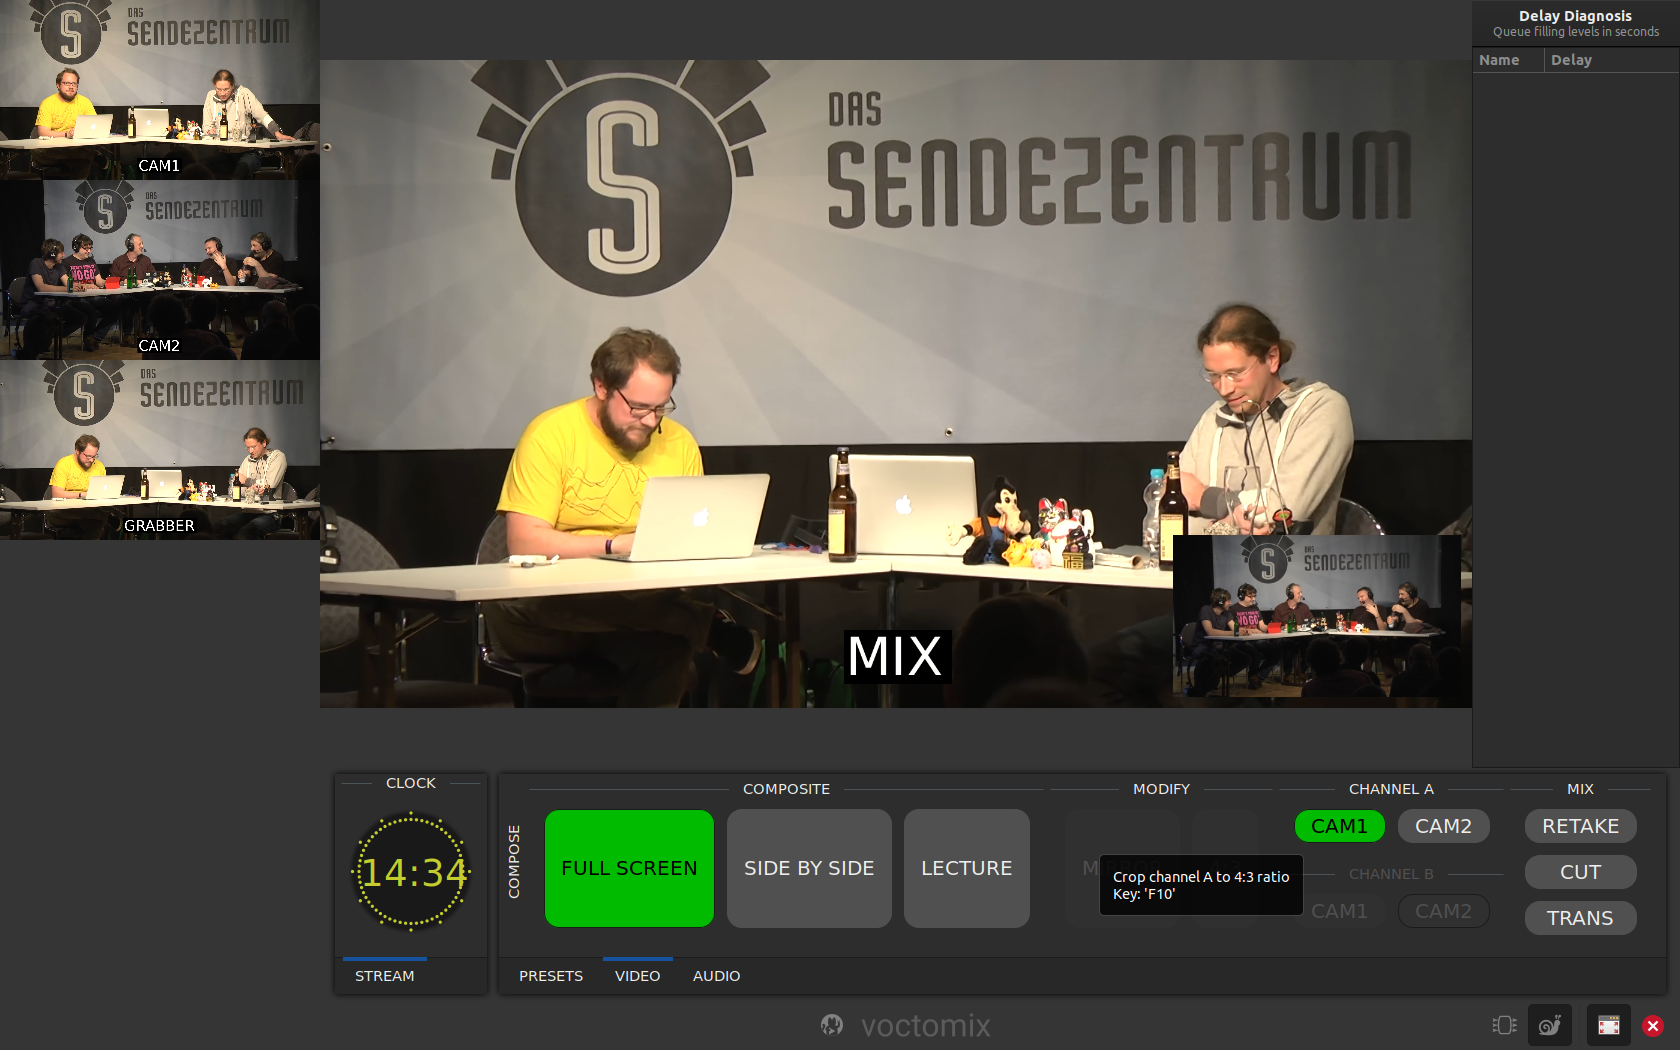
\includegraphics[width=\textwidth]{figuras/voctomix_inicial.png}
  \caption{Interfaz gráfica original de Voctomix al clonar el repositorio.}
  \label{fig:voctomix_inicial}
\end{figure}
